
\textbf{\underline{Четвертая глава}} раскрывает детали определения профиля опорной поверхности, на основе информации о точках её касания ногами робота и внутренних датчиков, характеризующих механическое состояние аппарата. Вторая часть главы показывает определение с помощью робота физико-механических свойств опорной поверхности:
жесткости, упругости и пластичности.

\textbf{Первая задача:} имеется поверхность. Каждому набору координат $x,\ y$ соответствует одно и только одно значение координаты $z$. Необходимо с помощью ощупывания роботом поверхности получить плотное облако точек и полигональную сетку. 

Сделано предположение, что расстояние между ногами робота мало относительно размеров поверхности, следовательно, поверхность между ногами считается плоскостью.

Для получения облака точек касаний опорных поверхностей, относительно глобальной системы координат, необходима трансформация систем координат от глобальной, до конкретного сенсора на ноге. Этому соответствует прямая задача кинематики \pic{fig:StriRus_10_legs_15_angle_v4.png}, \eqref{eq:forw_kin} и задачи локализации.

\begin{figure}[ht!]
    \centering
     \begin{tikzpicture}
        % Include the image in a node
        \node [above right, inner sep=0] (image) at (0,0) 
        {\centering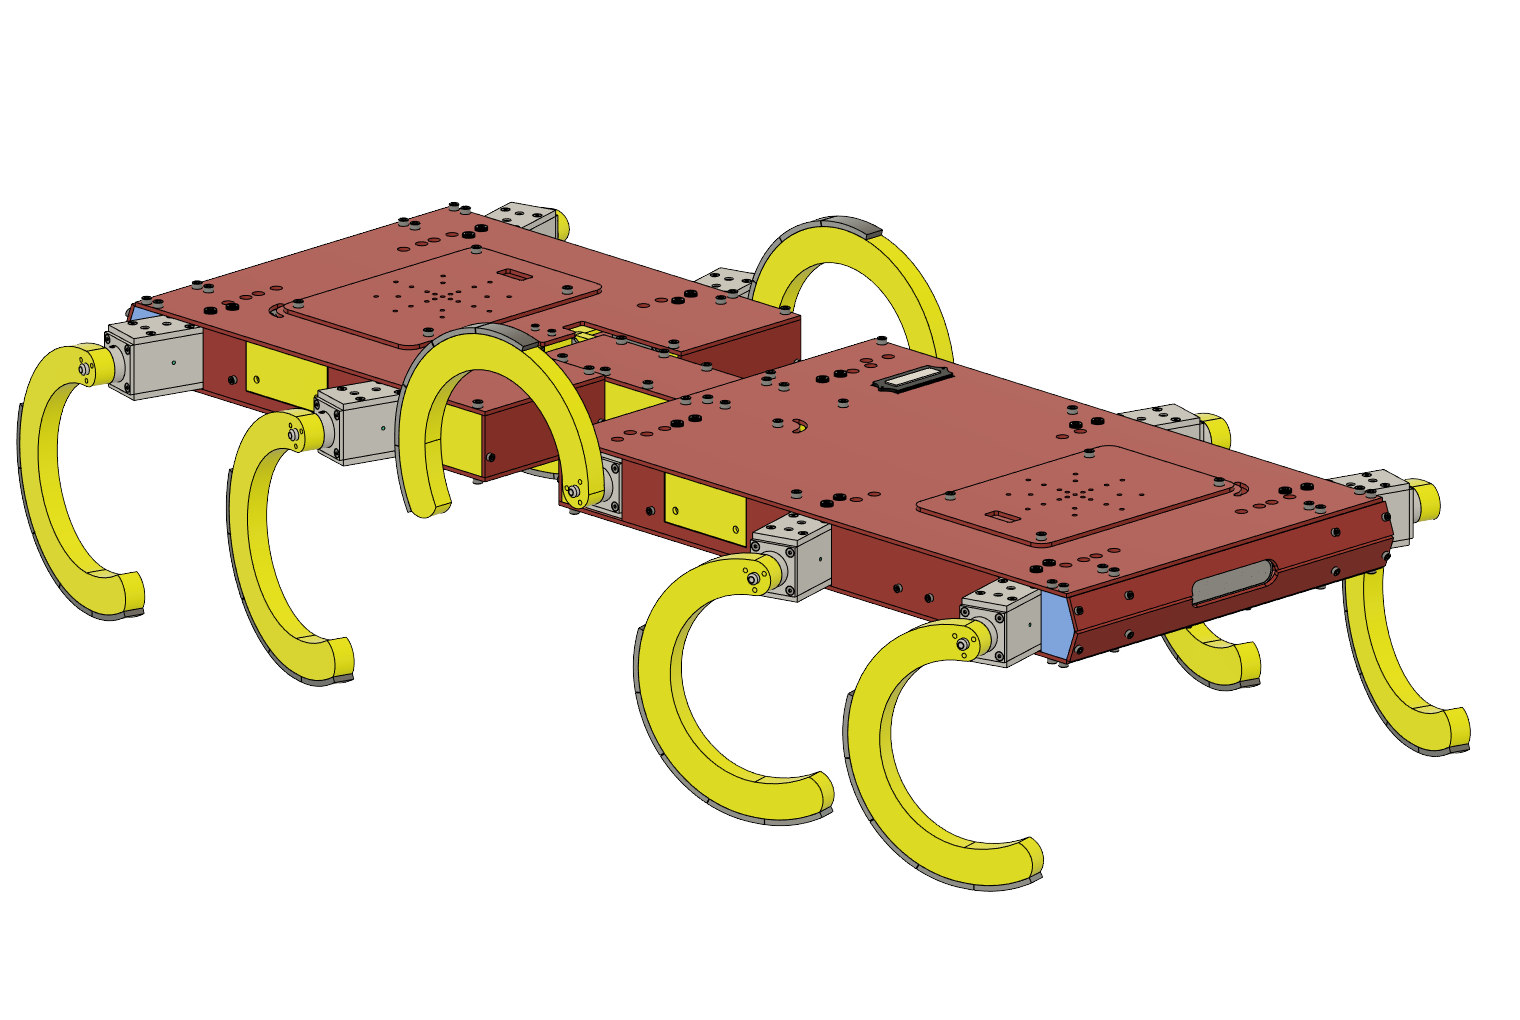
\includegraphics[height=5.5cm,width=1\textwidth,keepaspectratio]{StriRus_10_legs_15_angle_v4.png}};          
        % Create scope with normalized axes
        \begin{scope}[
            x={($ 0.1*(image.south east)$)},
            y={($ 0.1*(image.north west)$)}]
            % Grid and axes' labels
            % \draw[lightgray,step=1] (image.south west) grid (image.north east);
            % \foreach \x in {0,1,...,10} { \node [below] at (\x,0) {\x}; }
            % \foreach \y in {0,1,...,10} { \node [left] at (0,\y) {\y};}
 
            % Labels

            \coordinate (Xc) at (0.4415/2,-0.2347/2);
            \coordinate (Yc) at (-0.4512/2,-0.2156/2);
            \coordinate (Zc) at (0,0.5/2);
            % Labels
            \tikzstyle{origin} = [rounded corners=2pt, black, fill=gray!40, fill opacity=0.75, text opacity=1, scale=0.8,inner sep=1pt]
            \tikzstyle{transform_text} = [rounded corners=2pt, black, fill=white!85!gray, fill opacity=0.75, text opacity=1, scale=0.8,inner sep=1pt]
            \tikzstyle{transform_arrow} = [thick, green]
    
            % \coordinate (o_g) at (1,9);
            \node[circle,fill=green,scale=0.25] (o_g) at (1,9){};
            \draw[-stealth, very thick,blue] (o_g) -- ++(Xc);
            \draw[-stealth, very thick,green!70!black] (o_g) -- ++(Yc);
            \draw[-stealth, very thick,red] (o_g) -- ++(Zc);
            \node[origin,above right=3pt] at (o_g){\tiny $\mathbf{O_{glob}}$};
    
            % \coordinate (o_b) at (2.9,7.05);
            \node[circle,fill=green,scale=0.25] (o_b) at (2.9,7.05){};
            \draw[-stealth, very thick,blue] (o_b) -- ++(Xc);
            \draw[-stealth, very thick,green!70!black] (o_b) -- ++(Yc);
            \draw[-stealth, very thick,red] (o_b) -- ++(Zc);
            \node[origin,above right=2pt] at (o_b){\tiny $\mathbf{O_{base}}$};
    
            % \coordinate (o_1) at (2.9,6.6);
            \node[circle,fill=green,scale=0.25] (o_1) at (2.9,6.6){};
            \draw[-stealth, very thick,blue] (o_1) -- ++(Xc);
            \draw[-stealth, very thick,green!70!black] (o_1) -- ++(Yc);
            \draw[-stealth, very thick,red] (o_1) -- ++(Zc);
            \node[origin,above right=2pt] at (o_1){\tiny $\mathbf{O_{1}}$};
    
            % \coordinate (o_2) at (4,6);
            \node[circle,fill=green,scale=0.25] (o_2) at (4,6){};
            \draw[-stealth, very thick,blue] (o_2) -- ++(Xc);
            \draw[-stealth, very thick,green!70!black] (o_2) -- ++(Yc)
            node[origin,below=2pt]{\tiny $\mathbf{\alpha_3}$};
            \draw[-stealth, very thick,red] (o_2) -- ++(Zc);
            \node[origin,above right=2pt] at (o_2){\tiny $\mathbf{O_{2}=O_{3}}$};
    
            % \coordinate (o_4) at (7.0,4.55);
            \node[circle,fill=green,scale=0.25] (o_4) at (7.0,4.55){};
            \draw[-stealth, very thick,blue] (o_4) -- ++(Xc);
            \draw[-stealth, very thick,green!70!black] (o_4) -- ++(Yc);
            \draw[-stealth, very thick,red] (o_4) -- ++(Zc);
            \node[origin,above right=2pt] at (o_4){\tiny $\mathbf{O_{4}}$};
    
            % \coordinate (o_5) at (6.7,4.45);
            \node[circle,fill=green,scale=0.25] (o_5) at (6.7,4.45){};
            \draw[-stealth, very thick,blue] (o_5) -- ++(Xc);
            \draw[-stealth, very thick,green!70!black] (o_5) -- ++(Yc);
            \draw[-stealth, very thick,red] (o_5) -- ++(Zc);
            \node[origin,above left=3pt] at (o_5){\tiny $\mathbf{O_{5}=O_{6}}$};
    
            \coordinate (Xcr) at (0.49/2,0.07/2);
            % \coordinate (Ycr) at (-0.38/2,-0.32/2);
            \coordinate (Ycr) at (-0.24/2,-0.43/2);
    
            \draw[-stealth, very thick,blue] (o_5) -- ++(Xcr);
            \draw[-stealth, very thick,green!70!black] (o_5) -- ++(Ycr);
    
    
            % \coordinate (o_7) at (6.36,3.68);
            \node[circle,fill=green,scale=0.25] (o_7) at (6.36,3.68){};
            \draw[-stealth, very thick, blue] (o_7) -- ++(Xcr);
            \draw[-stealth, very thick, green!70!black] (o_7) -- ++(Ycr)
            node[origin,above left=2pt]{\tiny $\mathbf{\alpha_8}$};
            \draw[-stealth, very thick, red] (o_7) -- ++(Zc);
            \node[origin,below right=3pt] at (o_7){\tiny $\mathbf{O_{7}=O_{8}}$};
    
            \node[circle, draw ,fill=green,scale=0.4] (s_1) at (6.6,1.3){1};
            \node[circle,draw, fill=green,scale=0.4] (s_3) at (5.85,1.7){3};
            \node[circle,draw, fill=green,scale=0.4] (s_5) at (5.55,2.9){5};
    
            \draw[-stealth, transform_arrow] (o_g) -- (o_b)
            node[midway,below left=2pt, transform_text]{\tiny $\mathbf{H_{base}^{glob}}$};
    
            \draw[-stealth, transform_arrow] (o_b) -- (o_1)
            node[midway,left=3pt, transform_text]{\tiny $\mathbf{H_{1}^{base}}$};
    
            \draw[-stealth, transform_arrow] (o_1) -- (o_2)
            node[midway,below=2pt, transform_text]{\tiny $\mathbf{H_{2}^{1}}$};
    
            \draw[-stealth, transform_arrow] (o_2) -- (o_4)
            node[midway,below=2pt, transform_text]{\tiny $\mathbf{H_{4}^{3}}$};
    
            \draw[-stealth, transform_arrow] (o_4) -- (o_5)
            node[midway,below right=2pt, transform_text]{\tiny $\mathbf{H_{5}^{4}}$};
    
            \draw[-stealth, transform_arrow] (o_5) -- (o_7)
            node[midway,left=3pt, transform_text]{\tiny $\mathbf{H_{7}^{6}}$};
    
            \draw[-stealth, transform_arrow] (o_7) -- (s_1);
            \draw[-stealth, transform_arrow] (o_7) -- (s_3);
            \draw[-stealth, transform_arrow] (o_7) -- (s_5);
        \end{scope}
    \end{tikzpicture}
    \caption{Кинематическая схема для определения точки касания опорной поверхности роботом}
    \label{fig:StriRus_10_legs_15_angle_v4.png}
\end{figure}

\begin{multline}
    \label{eq:forw_kin}
        H_{leg}^{glob} = H(x_{glob},y_{glob},z_{glob},\alpha_{glob},\beta_{glob},\gamma_{glob})T_z(l_1)\\ T_x(l_2)R_y(\alpha_3)T_x(l_4)T_y(l_5)R_z(-15^{\circ})T_y(l_7)R_y(\alpha_8)
\end{multline}
Где каждая матрица представляет собой матрицу однородного преобразования, через $R_i$ обозначены однородные матрицы поворота, относительно соответствующей осеи, $T_i$ --- однородную матрицу перемещения.

Для получения плотного облака точек необходимо очистить оригинальное облако точек от шумов и усреднить близлежащие точки с помощью Voxel grid. Потом из него генерируется полигональная сетка с помощью 2D Триангуляции Делоне \pic{fig:delone_idea.png} (вогнутая оболочка \pic{fig:exp_concave_hull}). На ее основе получается необходимое плотное облако точек. 

\begin{figure}[ht!]
    \centering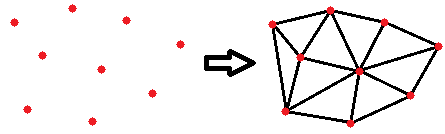
\includegraphics[height=2.5cm,width=1\textwidth,keepaspectratio]{delone_idea.png}
    \caption{2D Триангуляция Делоне (выпуклая оболочка)}
    \label{fig:delone_idea.png}
\end{figure}

Модификация триангуляции Делоне нужна, так как выпуклой оболочке \pic{fig:conv_convex.png} алгоритм построил карту местности там, где робот не ходил. При использовании вогнутой оболочки \pic{fig:conv_concave.png} данная проблема не наблюдается.

\begin{figure}[H]
    \begin{subfigure}[t]{0.32\textwidth}
        \centering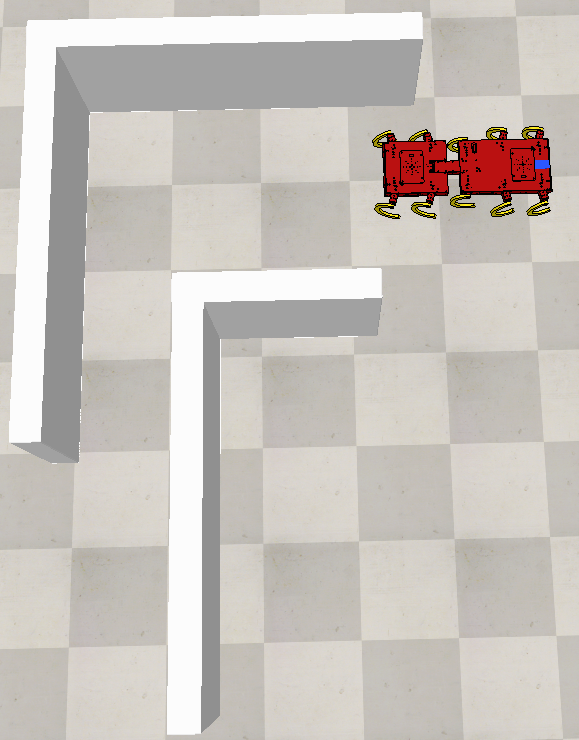
\includegraphics[height=3cm,width=1\textwidth,keepaspectratio]{convex_terr.png}
        \caption{Пример поля}
        \label{fig:convex_terr.png}
    \end{subfigure}
    \begin{subfigure}[t]{0.32\textwidth}
        \centering
        \begin{tikzpicture}
            % Include the image in a node
            \node [above right, inner sep=0] (image) at (0,0)
            {\centering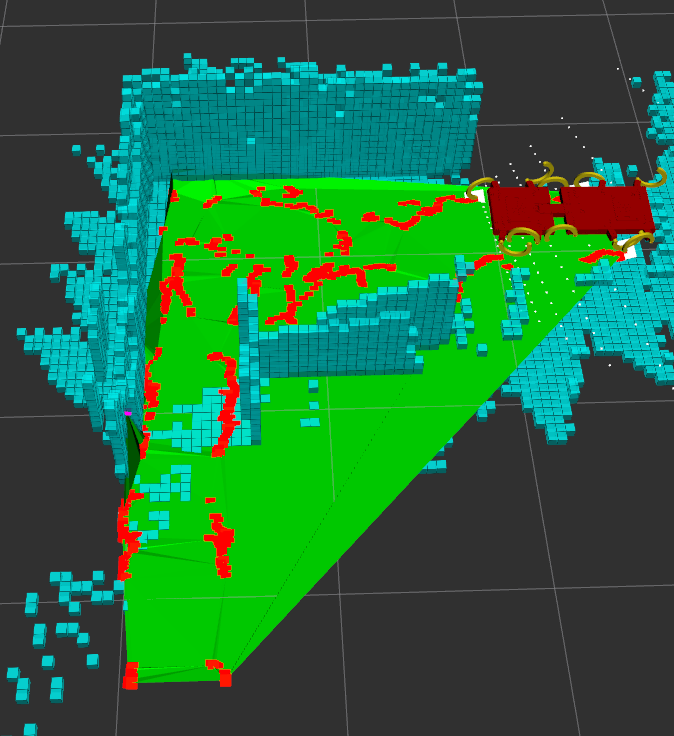
\includegraphics[height=4cm,width=1\textwidth,keepaspectratio]{conv_convex.png}};
            % Create scope with normalized axes
            \begin{scope}[
                x={($ 0.1*(image.south east)$)},
                y={($ 0.1*(image.north west)$)}]
            % Labels
            \draw[stealth-, very thick,green] (5.2,3.5) -- ++(0,-1)
            node[rounded corners=3pt,right,black,fill=white]{\tiny Полученная сетка};

            \draw[stealth-, very thick,green] (5.5,5.5) -- (6.4,4)
            node[rounded corners=3pt,right,black,fill=white]{\tiny Данные лидара};


            \draw[stealth-, very thick,green] (3.4,0.8) -- (5,1);
            \draw[stealth-, very thick,green] (3.4,2.6) -- (5,1)
            node[rounded corners=3pt,right,black,fill=white]{\tiny Следовая дорожка};
        \end{scope}
        \end{tikzpicture}
        \caption{Выпуклая оболочка}
        \label{fig:conv_convex.png}
    \end{subfigure}
    \begin{subfigure}[t]{0.32\textwidth}
        \centering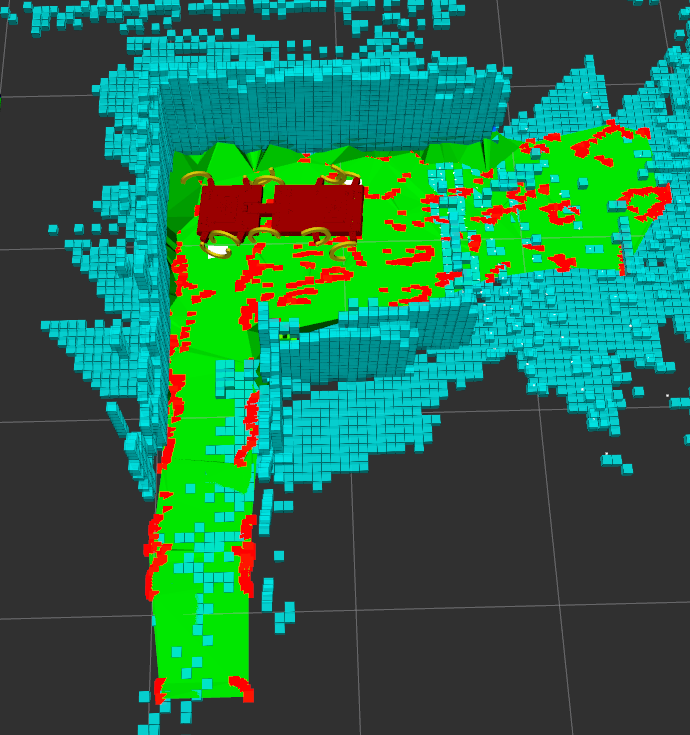
\includegraphics[height=4cm,width=1\textwidth,keepaspectratio]{conv_concave.png}
        \caption{Вогнутая оболочка}
        \label{fig:conv_concave.png}
    \end{subfigure}
    \caption{Объяснение необходимости модификации алгоритма Делоне}
    \label{fig:exp_concave_hull}
\end{figure}

Проверка алгоритма в симуляции (Рис. \ref{fig:unsolvable_case}), натурно \pic{fig:real_exp_map_creation}.

\begin{figure}[H]
    \begin{subfigure}[t]{0.49\textwidth}
            \centering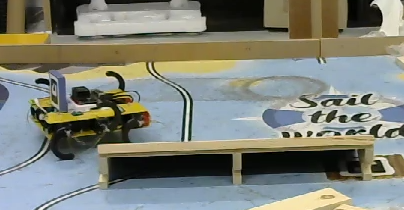
\includegraphics[height=6cm,width=1\textwidth,keepaspectratio]{real_robot_mesh_video_preview.png}
        \caption{Робот проходит препятствие}
        \label{fig:real_robot_mesh_video_preview.png}
    \end{subfigure}
    \begin{subfigure}[t]{0.49\textwidth}
        \centering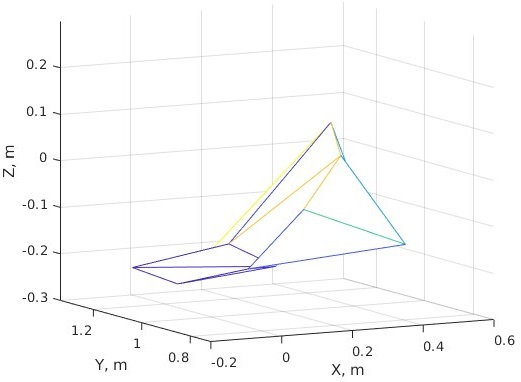
\includegraphics[height=3cm,width=1\textwidth,keepaspectratio]{real_mesh.jpg}
        \caption{Полученная полигональная сетка}
        \label{fig:real_mesh.jpg}
    \end{subfigure}
    \caption{Пример натурного эксперимента}
    \label{fig:real_exp_map_creation}
\end{figure}

Для оценки точности полученных данных использовались метрики Cloud to Cloud (C2C) \eqref{eqn:hauff} и Cloud to Mesh (C2M) \pic{fig:metrics}.

\begin{equation}
    \label{eqn:hauff}
    d_{H}(X,\;Y)=\sup _{m\in M}\left\{\,|\mathrm {dist} _{X}(m)-\mathrm {dist} _{Y}(m)|\,\right\}    
\end{equation}
Где $X,\ Y$ непустые подмножества метрического пространства $M$; $\mathrm {dist} _{X}\colon M\to \mathbb {R}$ $\mathrm {dist} _{X}\colon M\to \mathbb {R}$ обозначает функцию расстояния до множества $X$.


\begin{figure}[ht!]
    \begin{subfigure}[t]{0.49\textwidth}
        \centering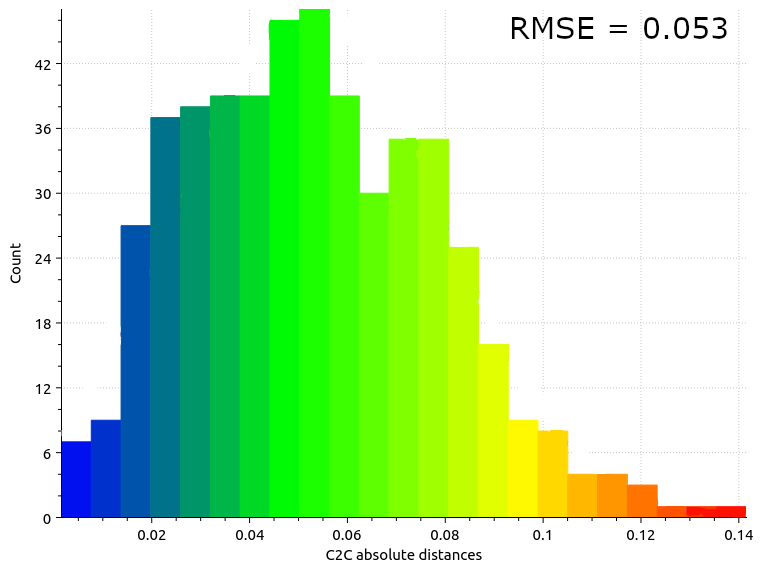
\includegraphics[height=3.5cm,width=1\textwidth,keepaspectratio]{pcd_hist.png}
        \caption{Метрика C2C: гистограмма ошибок (абсолютное расстояние от точки до ближайшей реферальной точки)}
        \label{fig:metric_c2c}
    \end{subfigure}
    \begin{subfigure}[t]{0.49\textwidth}
        \centering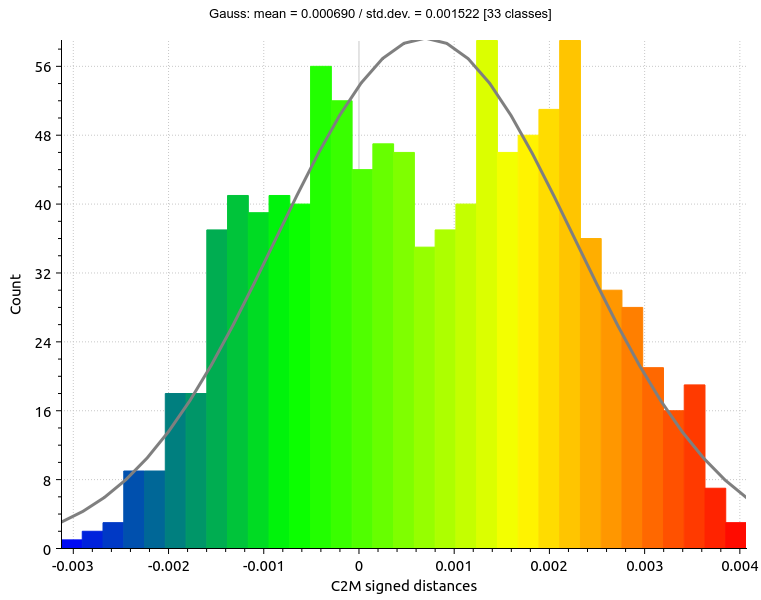
\includegraphics[height=3.5cm,width=1\textwidth,keepaspectratio]{mesh_hist.png}
        \caption{Метрика C2M: Гистограмма ошибок (относительное расстояние от точки до ближайшей реферальной точки)}
        \label{fig:metric_c2m}
    \end{subfigure}
    \caption{Метрики оценки точности полученной карты}
    \label{fig:metrics}
\end{figure}


Как итог, среднеквадратичная ошибка для C2C метрики была в среднем равна 5 см. А для C2M 1 см. В натурном эксперименте по метрике C2C --- 8 см.

\textbf{Вторая задача} это определение физико-механических свойств опорной поверхности. С точки зрения механики свойства поверхности с водятся к показателям упругости, вязкости и пластичности. Однако непосредственное измерение этих показателей затруднительно. В исследовании решалась задача классификации опорной поверхности с помощью искусственной нейронной сети. В качестве эталона жёсткой поверхности использовались крупные камни, эталоном упругой поверхности была принята резина, а эталоном поверхности с явно выраженными свойствами пластичности выступила песчаная почва. 

При движении робота по поверхности собираются данные с датчиков силы и с моторов. На основе предварительного обучения с помощью метода опорных векторов (SVM), данные обрабатываются и классифицируется.

Вектор с входными данными представлен следующим образом:
\begin{itemize}
    \item Элемент(1) --- Частота движения ног
    \item (2) --- Пиковая амплитуда давления с датчика силы
    \item (3) --- Ширина давления с датчика силы. Это расстояние между началом и концом акта движения. Такие отрезки складываются и получается ширина.
    \item (4) --- Площадь под кривой силы датчика
    \item (5) --- Пиковая амплитуда крутящего момента двигателя
    \item (6) --- Пиковый крутящий момент двигателя
    \item (7) --- Среднее давление на сенсорах
    \item (8) --- Средняя амплитуда крутящего момента
    \item (9) --- Средний крутящий момент двигателя
    \item (10) --- Ширина крутящего момента двигателя
    \item (11) --- Площадь под кривой крутящего момента двигателя
    \item (12-16) --- Индивидуальная пиковая амплитуда силы датчика силы 
\end{itemize}

В качестве причин выбора таких входных данных можно отметить следующие. Видно различное поведение сенсоров в зависимости от типа поверхности \pic{fig:s_shape_leg/TaxelIndForce_full.png}. Зависимость средней линейной скорости движения ноги на разных поверхностях при различных угловых скоростях \pic{fig:s_shape_leg/avg_lin_vel_rev_min.png}. 


\begin{figure}[ht!]
    \begin{subfigure}{0.99\textwidth}
        \centering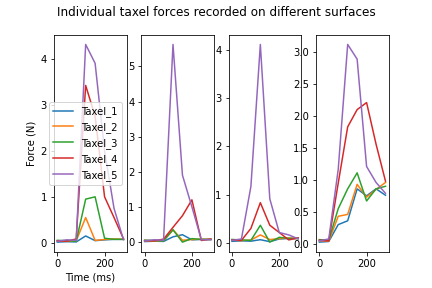
\includegraphics[height=4.5cm,width=1\textwidth,keepaspectratio]{s_shape_leg/TaxelIndForce.png}
        \caption{Запись активных датчиков силы на разных поверхностях}
        \label{fig:s_shape_leg/TaxelIndForce_full.png}
    \end{subfigure}

    \begin{subfigure}{0.99\textwidth}
        \centering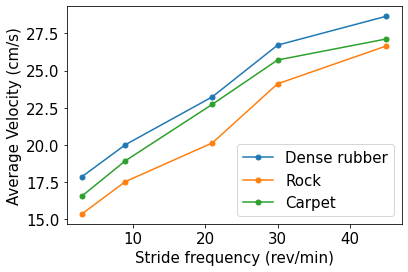
\includegraphics[height=3.5cm,width=1\textwidth,keepaspectratio]{s_shape_leg/avg_lin_vel_rev_min.png}
        \caption{Средняя линейная скорость робота}
        \label{fig:s_shape_leg/avg_lin_vel_rev_min.png}
    \end{subfigure}

\caption{Причины использования конкретных входных данных}
\end{figure}

В процессе обучения собранные данные были разделены на обучающее (80\% данных) и тестовое множества (20\%). Модель была обучена с использованием ядра на основе функции Пирсона VII (PUK). 

Для оценки эффективности модели использовался тестовый набор. Производительность измерялась с точки зрения точности классификации и F1-score.

Функция принятия решения для SVM-модели \eqref{eq:SVM}:

\begin{align}
    \label{eq:SVM}
    f(x) = w^T x + b
\end{align}

где $x$ --- входной вектор, $w$ является весовым вектором, и $b$ --- смещение.

Универсальное ядро на основе функции Пирсона VII \eqref{eq:PUK}:

\begin{align}
    \label{eq:PUK}
    K(x, y) = (1 + ((||x - y||^2)/\sigma^2)^\omega)^{(-1/\omega)}
\end{align}
Где $x$, $y$ --- векторы во входном пространстве, $||x - y|||$ обозначает евклидово расстояние между $x$ и $y$, $\sigma$ --- масштабный параметр, определяющий <<разброс>> ядра, $\omega$ --- это параметр формы, который влияет на форму границы принятия решения.

Данные собирались с установки, которая разрабатывалась так, чтобы было возможно быстро сменить тип поверхности, нога робота бесконечно могла совершать движения и узел с ногой был таким же как на реальном роботе \pic{fig:s_shape_leg/s_leg_setup.JPG}.

\begin{figure}[H]
    \begin{subfigure}{0.39\textwidth}
        \centering
        \begin{tikzpicture}
            % Include the image in a node
            \node [above right, inner sep=0] (image) at (0,0)
            {\centering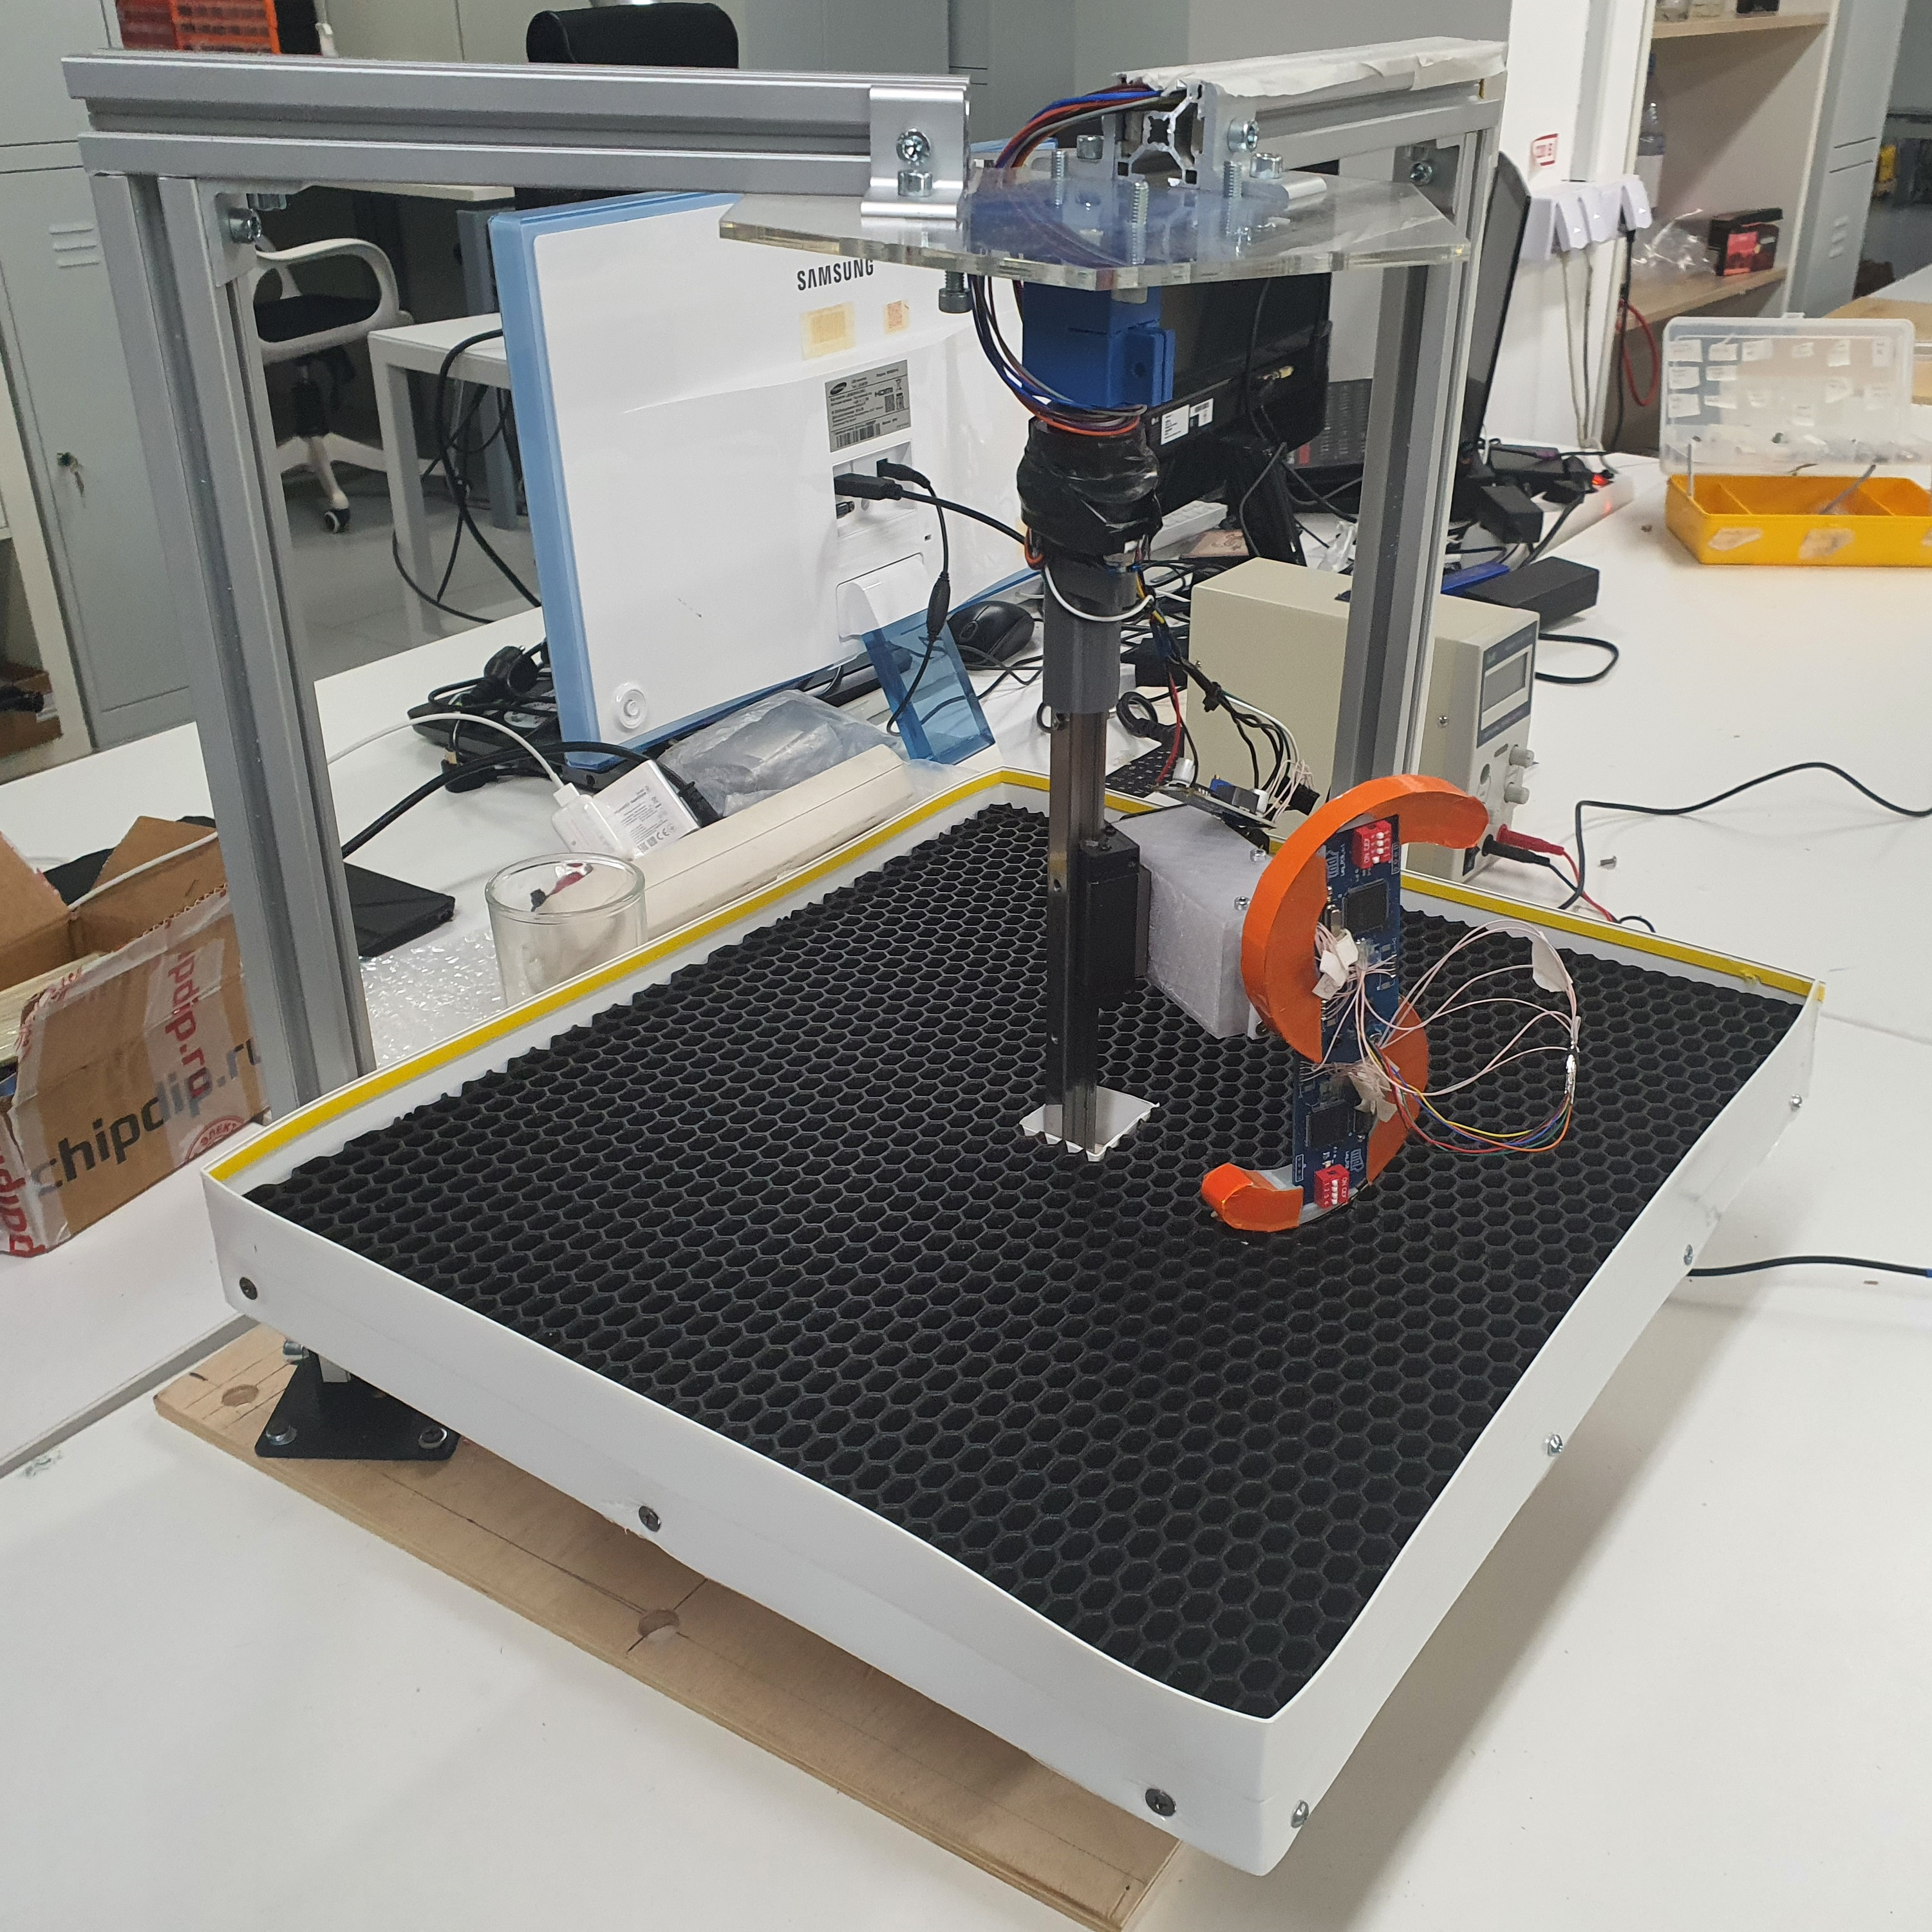
\includegraphics[height=5cm,width=1\textwidth,keepaspectratio]{s_shape_leg/s_leg_setup.JPG}};
            % Create scope with normalized axes
            \begin{scope}[
                x={($ 0.1*(image.south east)$)},
                y={($ 0.1*(image.north west)$)}]
            \draw[stealth-, very thick,green] (3.5,2.5) -- (3,1.5)
            node[rounded corners=3pt,below,black,fill=white]{\tiny Стол для поверхностей};
    
            \draw[stealth-, very thick,green] (7.1,5.4) -- (7.4,7)
            node[rounded corners=3pt,above right,black,fill=white]{\tiny Контроллер};
    
            \draw[very thick,green] (6,6.1) rectangle (8.5,3.5)
            node[above left,black,fill=green]{\tiny S leg};
        \end{scope}
        \end{tikzpicture}
        \caption{Общий вид экспериментальной установки}
    \end{subfigure}
        \begin{subfigure}{0.20\textwidth}
            \centering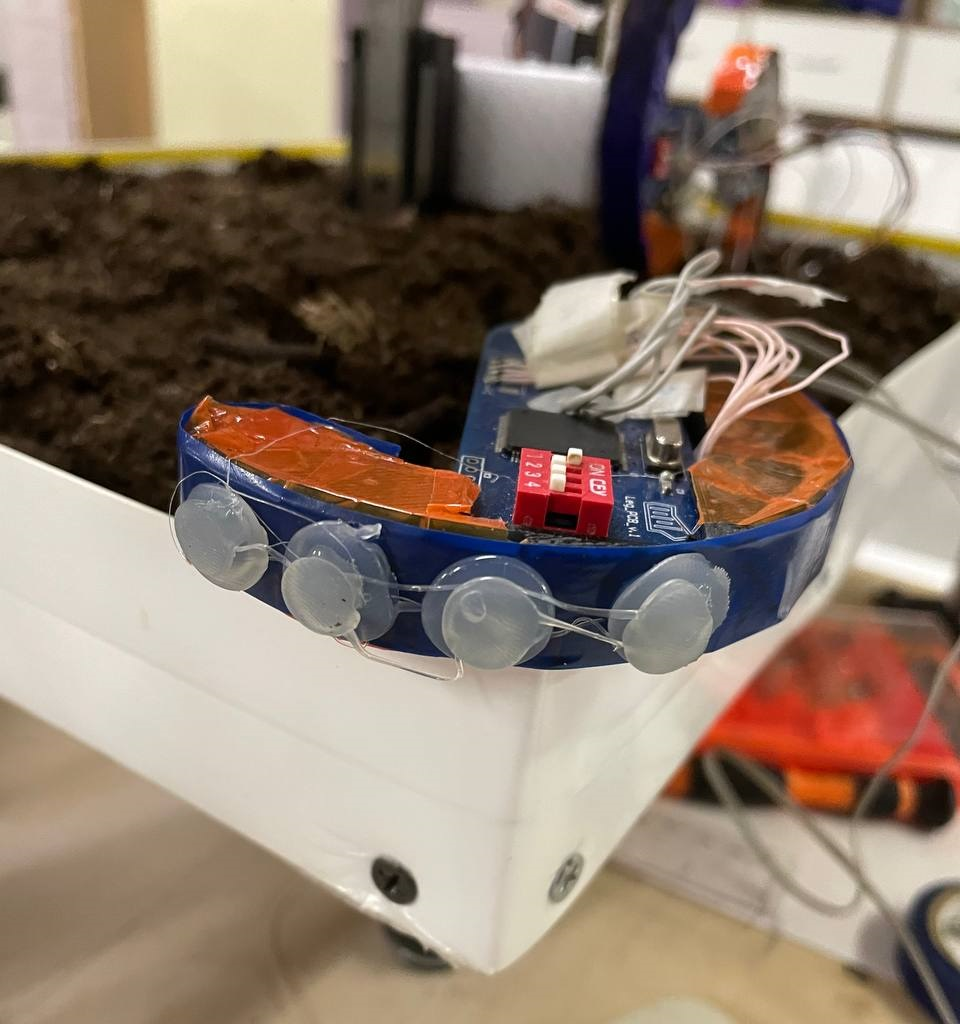
\includegraphics[height=5cm,width=1\textwidth,keepaspectratio]{s_shape_leg/socks_new.jpg}
            \caption{Расположение сенсоров на ноге робота}
            \label{fig:s_shape_leg/socks.jpg}
        \end{subfigure}
        \begin{subfigure}{0.39\textwidth}
            \centering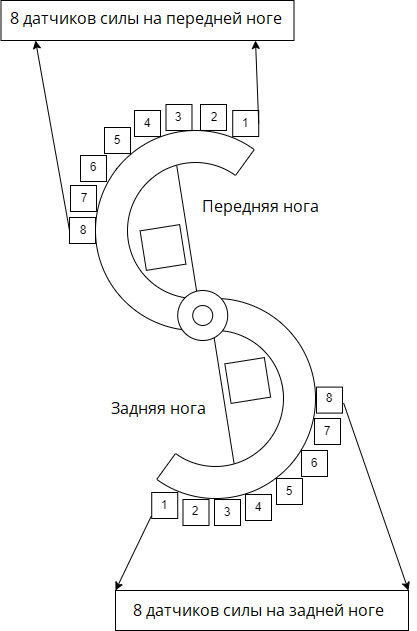
\includegraphics[height=5cm,width=1\textwidth,keepaspectratio]{s_shape_leg/leg_design.png}
            \caption{Схематическое расположение сенсоров на ноге установки}
            \label{fig:s_shape_leg/leg_design.png}
        \end{subfigure}

    \caption{Экспериментальная установка}
    \label{fig:s_shape_leg/s_leg_setup.JPG}
\end{figure}


Результат обучения представлен в виде таблицы \tab{tabular:prob_terrain_classification}.

\begin{table}[H]
    \caption{Вероятность определения типа поверхности}
    \label{tabular:prob_terrain_classification}
    \centering
\begin{tabular}{|c|c|c|c|c|} 
    \cline{3-5}
    \multicolumn{1}{l}{} & \multicolumn{1}{l|}{} & \multicolumn{3}{c|}{\textbf{Предсказанный класс}} \\ 
    \cline{3-5}
    \multicolumn{1}{l}{} &  & Камень & Резина & Земля \\ 
    \hline
    \multirow{3}{*}{{\textbf{Истинный класс}}} & Камень & {\cellcolor[rgb]{0.741,0.843,0.929}}84.0\% & 2.56\% & 13.44\% \\ 
    \hhline{|~----|}
     & Резина & 20.1\% & {\cellcolor[rgb]{0.741,0.843,0.929}}67.8\% & 12.1\% \\ 
    \hhline{|~----|}
     & Земля & 1.0\% & 18.9\% & {\cellcolor[rgb]{0.741,0.843,0.929}}80.1\% \\
    \hline
    \end{tabular}
\end{table}

Полученные результаты показывают, что в подавляющем большинстве случаев, удаётся корректно определить класс опорной поверхности. Ошибочные результаты классификации как правило не являются критичными, поскольку определение класса поверхности при движении робота осуществляется многократно в каждой точке касания. И, например, ошибка 20 \% при определении класса означает, что в среднем в каждой пятой точке касания робот будет определять поверхность как более жёсткую, чем она есть на самом деле.

Разработанный метод определения физико-механических свойств поверхности показал достаточно высокий результат классификации поверхностей по трём классам, и может быть применим для более детальной классификации.